\newpage
{\bfseries ҒТАMР 52.35.29}
\hfill {\bfseries \href{https://doi.org/10.58805/kazutb.v.2.23-254}{https://doi.org/10.58805/kazutb.v.2.23-254}}

\sectionwithauthors{М.С.Усенбеков, Е.М. Мейрам, М.Н. Жумабеков, М. Рабатұлы, Т.К. Исабек}{КӨМІР ҚАБАТЫНДАҒЫ ЖЕРАСТЫ ГАЗСЫЗДАНДЫРУ ҰҢҒЫМАЛАРЫНАН ГАЗ ШЫҒУЫН АРТТЫРУ}

\begin{center}
{\bfseries М.С.Усенбеков\textsuperscript{🖂}, Е.М. Мейрам, М.Н. Жумабеков, М. Рабатұлы, Т.К. Исабек}

Әбілқас Сағынов атындағы Қарағанды техникалық университеті, Қарағанды,
Қазақстан,

{\bfseries \textsuperscript{🖂}} Корреспондент-автор: meirambek46@mail.ru
\end{center}

Бұл жұмыста қабаттың газ шығуын арттыру үшін көмір қабатын гидравликалық
айыру әдісін қолдану нәтижелері келтірілген. Бұл ретте диаметрі 93 мм
және ұзындығы 40-80 метр ұңғымалар арқылы 300 атм аспайтын қысыммен
пакерлер арқылы шахта суы айдалды. Гидравликалық айыру әдісіне дейін
және одан кейін ұңғымалардың аузындағы өлшеулер көмір қабатынан газ
шығуының орта есеппен 1,8 есе артқанын көрсетті.

{\bfseries Түйін сөздер:} көмір қабаты, газ шығуы, гидравликалық айыру
әдісі, шахта, ұңғыма, жарықшалар, метан.

\begin{center}
{\large\bfseries INCREASING THE GAS OUTPUT OF UNDERGROUND DEGASSING WELLS IN THE
COAL SEAM}

{\bfseries M.S.\textsuperscript{.}Usenbekov\textsuperscript{🖂}, E.M.
Meiram, M.N.Zhumabekov, M.Rabatuly, T.K.Isabek}

Abylkas Saginov Karaganda Technical University, Karaganda, Kazakhstan,

e-mail: meirambek46@mail.ru
\end{center}

This paper presents the results of the application of hydraulic
fracturing of a coal seam to increase its gas recovery. At the same
time, mine water was pumped through wells with a diameter of 93 mm and a
length of 40-80 meters at a pressure of no more than 300 atm through
packers. Measurements at the wellhead before and after hydraulic
fracturing showed an increase in coal seam gas recovery by an average of
1.8 times.

{\bfseries Keywords:} coal seam, gas release, hydraulic fracturing, mine,
well, fractures, methane

\begin{center}
{\large\bfseries ПОВЫШЕНИЯ ГАЗООТДАЧИ ПОДЗЕМНЫХ ДЕГАЗАЦИОННЫХ СКВАЖИН В УГОЛЬНО
ПЛАСТЕ}

{\bfseries М.С.Усенбеков\textsuperscript{🖂}, Е.М.Мейрам, М.Н.Жумабеков,
М.Рабатұлы, Т.К.Исабек}

Карагандинский технический университет им. Абылкаса Сагинова, Караганда,
Казахстан,

е-mail: meirambek46@mail.ru
\end{center}

В данной работе приведены результаты применения гидроразрыва угольного
пласта для повышения его газоотдачи. При этом через скважины диаметром
93 мм и длиной 40-80 метров под давлением не более 300 атм через пакеры
закачивалась шахтная вода. Замеры на устье скважин до и после
гидроразрыва показали увеличение газоотдачи угольного пласта в среднем в
1,8 раза.

{\bfseries Ключевые слова:} угольный пласт, газовыделение, гидравлический
разрыв, шахта, скважина, трещины, метан.

\begin{multicols}{2}
{\bfseries Кіріспе.} Көмір қабаттарын игеру тереңдігінің артуымен
газ-динамикалық құбылыстардың қаупі жоғарылап, кенжарға газ шығарудың
артуы байқалады, бұл көмір өндіру қарқынын тежейді және тау-кен
жұмыстарының қауіпсіздігін төмендетеді. Көмір метанның белгілі бір
мөлшерін тиісті қысым мен температурада байланыстырылған күйде ұстай
алады. Көмірден метанды алу сорбциялық тепе-теңдік бұзылған және газ
ұңғымаларға қарай жылжитын көміртегі массивінің өткізгіштігі жоғарылаған
жағдайда ғана мүмкін болады.

Әлемдік тәжірибеде газсыздандыруды қарқындату әдістерін талдау көмір
қабаттарының газ шығару қабылетін өсіру үшін қабатты гидравликалық айыру
әдісін (ҚГАӘ) жиі қолданылатынын көрсетеді {[}1,2,3,4{]}. ҚГАӘ
процесінде пайда болған жарықшалар ұзындығы бірнеше ондаған метрге жетуі
мүмкін, бір-бірімен және басқа жарықшалармен байланысып, массивтің
өткізгіштігін едәуір арттырады. Бұл әдіс бүгінгі күнге дейін
ұңғымалардан газ шығуын арттырудың ең тиімді әдісі болып табылады
{[}5,6,7,8{]}.

Шахта жағдайында гидравликалық айыру әдісі көмір қабатын газсыздандыру
мерзімдерін азайту мақсатында және көмір қабаттарының алдын-ала
газсыздандыру дәрежесін арттыру үшін қолданылады. Оның мәні көмір
қабатында тау жыныстарының массивін ішінара түсіруге, онда тау
жыныстарын газсыздандыру үшін сүзгі арналарын құруға арналған жарықтар
жүйесін қалыптастырудан тұрады.

{\bfseries Материалдар мен әдістер.} Қазіргі уақытта көмір қабатын игеру
алдында конвейерлік және желдету штректері маңында бұрғыланған ұңғымалар
арқылы алдын ала газсыздандыру жүргізіледі, содан кейін оларды 6 ай бойы
вакуумдық сорғы станциясына қосады. Бұл әдістің кемшілігі ұңғымалардың
қабырғалары арқылы ұңғыма маңындағы көмір қабатының өте кішкентай
аймағынан газ шығарылады. Сондықтан көмір қабаттарынан газды бұл әдіспен
алу тиімділігі осы жағдайларда қауіпсіз жұмысты қамтамасыз ету үшін
жеткіліксіз {[}9{]}. Көмір қабатының газдылығын төмендетудің негізгі
әдісі - газсыздандыру ұңғымаларын дайындық қазбаларынан қазба бағанының
денесіне бұрғылау. Тәжірибе көрсеткендей, белсенді газ шығару кезеңі
және жалпы газсыздандыру ұңғымасының тиімділігі өте аз, бұл қабаттың
физика-механикалық қасиеттеріне байланысты. Көмір қабатын ұңғыма арқылы
газ шығару процесін гидроайыру жарықшақтарын қалыптастыру арқылы оған
қосымша әсер ету беттерін жасау арқылы күшейтуге болады. Көмір қабатының
газ шығынын арттыру арқылы алдын ала газсыздандырудың тиімділігін
арттыру үшін жақында көмір массивінің гидроайыруы қолданылады. Көмір
қабатын ұңғыма арқылы газ шығару процесін гидроайыру жарықтарын
қалыптастыру арқылы оған қосымша әсер ету беттерін жасау арқылы
күшейтуге болады.
\end{multicols}

\begin{figure}[H]
	\centering
	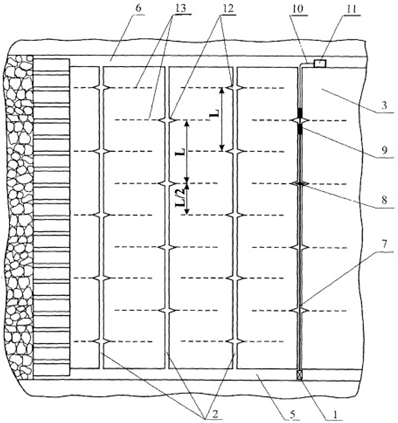
\includegraphics[width=0.5\textwidth]{assets/1133}
	\caption*{1-сурет - Гидравликалық айыру әдісімен газдың шығыуын ұлғайту схемасы:}
	\caption*{1-станок; 2-ұңғыма; 3-көмір массиві; 4-тазарту кенжары; 5-конвейер
штрегі; 6- желдету штрегі; 7-бұрғылау қондырғы; 8-саңылау түзгіш;
9-тығыздағыш құрылғы; 10-құбыр; 11-сорғы станциясы; 12-инициативті
саңылау; 13-гидроайыру жарықшақтары; L-саңылау түзгіштер аралығы}
\end{figure}

\begin{multicols}{2}
Гидравликалық айыру әдісін орындау үшін арнайы бұрғыланған жерасты
ұңғымаларын қолданады. Станок 1 (1-сурет) бұрғыланған көмір массивіндегі
3 ұңғымаларды 2 контурлау қазбаларынан тазарту кенжарына 4 параллель
бұрғылайды, мысалы, конвейер штрегінен 5 желдету штрегіне 6 дейін. Содан
кейін конвейерлік штрек 5 жағынан ұңғымада 2 бұрғылау қондырғысы бар
жабдықты 7, тығыздағыш 9 құрылғысы бар саңылаутүзгішті 8 монтаждау
жүргізіледі. Икемді құбыр 10 арқылы тығыздағыш құрылғы 9 желдеткіш
штректе 6 орналасқан сорғы станциясына 11 қосылады. Әрі қарай, конвейер
штрегінің 5 жағында бастаушы саңылаулар 12 кесіліп, тығыздағыш құрылғы 9
бен саңылау түзгіштің 8 ұзындығының қосындысына тең әрі L-қадаммен
саңылаулар түзеді. Бұл әрбір келесі бастау саңылауын 12 кесу кезінде
әрбір алдыңғы саңылаутүзушіні тығыздауға және айыруға мүмкіндік береді,
бұл саңылаутүзушіні кесу және гидроайыру операцияларын біріктіруге
мүмкіндік береді. Сорғы станциясының 11 кесілген инициативті
саңылауларын 12 икемді құбыр 10 арқылы қысыммен тығыздағыш құрылғыға 9
айыру үшін жұмыс сұйықтығы беріледі - инициативті саңылау 12 орналасқан
ұңғыма аймағы тығыздалады. Тығыздағыш құрылғы 9 орнатылған қысым
деңгейінен асып кеткен кезде, жұмыс сұйықтығы инициативті саңылауға 12
жіберіледі және гидроайыру жарықшақтары пайда болады.

Көмір массивін 3 гидроайыру бойынша жұмыстар аяқталғаннан кейін бірінші
ұңғыманың 2 бүкіл ұзындығы бойынша оған іргелес келесі ұңғымадағы 2
ұқсас жұмыстарға ауысады, бұл ретте инициативті саңылауларды 12 кесу сол
әдіспен және L кесу қадамымен жүргізіледі. Алайда, кейінгі ұңғымадағы 2
инициативті саңылауларды 12 кесу алдыңғы ұңғыманың 2 инициативті
саңылауларына 12 қатысты кесу қадамын инициативті саңылаулар 12
арасындағы қашықтықтың жартысына тең шамаға ауыстыра отырып жүзеге
асырылады. Осылайша, іргелес ұңғымалардың көмір массивінің гидроайыру
жарықшақтары 13 арасындағы қашықтық екі есе азаяды және L/2-ге (1-сурет)
тең болады, сондықтан көмір массивінің әсер ету аймағы екі есе көп
болады, бұл көмір қабатын кейінгі газсыздандыру тиімділігін арттырады.

Кейінгі ұңғымалар 2 бірдей ретпен өңделеді. Бұл ретте бұрғыланған
ұңғымаларда оның бүйір бетіндегі инициативті саңылаулар кесіледі,
ұңғыманың үзілу аралығы арнайы пакермен тығыздалады, содан кейін көмірде
жарықшақтар пайда болуы үшін қысыммен суды үзіліс аралығына айдайды. Бұл
жағдайда инициативті саңылауды кесу кезінде пайда болған көмір
бөлшектері ұңғыманың үзілу аралығында ұсталады, айдалатын сумен
араластырылады және алынған суспензия жарықшаққа айдалады. Техникалық
нәтиже - газды көмір қабаттарын газсыздандыру тиімділігін арттыру болып
табылады.

Гидравликалық айыру әдісі диаметрі 93 мм, ұзындығы 40-80 метр
ұңғымаларда іске асырылды. Гидравликалық айыру ұңғымалары мен
газсыздандыру ұңғымалары судың айыру процесі тоқтағаннан кейін
газсыздандыру желісіне қосылды. ҚГАӘ-ның тиімділігі метанның шығуының
өсуіне дейін және одан кейін өлшенген дебиттерін салыстыру арқылы
анықталды. Сонымен қатар, «Казахстанская» шахтасында қабат ұңғымаларын
газсыздандыру желісіне қосу 10 ұңғымадан блокпен жүргізілді, онда ҚГАӘ
қолданумен немесе қолданусыз аудандарда метан дебиттеріне салыстыру
жүргізілді.

Қабатты гидравликалық айыру сорғының көмегімен шамамен 16 МПа қысыммен
айдалатын жұмыс сұйықтығымен жүзеге асырылады. Жұмыс сұйықтығы ретінде
шахта су құбырының суы қолданды {[}10{]}.

Қабатты гидравликалық айыру сұйықтықтың берілген көлемін қабатқа
айдағаннан кейін немесе оның штрек қабырғасында пайда болғаннан кейін
тоқтатылады. Көмір қабатын газсыздандыру схемасы суретте келтірілген.

ҚГАӘ бойынша жұмыстардың құрамына мынадай негізгі операциялар кіреді:

- ҚГАӘ өндірісіне дейін ұңғымалардан метан дебитін өлшеу;

- сорғы жабдығын ұңғымаға қосқанға дейін сынау;

- жабдықты 16 МПа астам қысыммен престеу;

- жұмысқа сорғы жабдықтарын қосу;

- айдау қысымын, пакердегі қысымды және жұмыс сұйықтығын айдау көлемін
бақылау.

Қолданылатын құрал-жабдықтар:

1. Су айдауға арналған сорғы УНИ:

- 50 л/мин су шығымы;

- максималды қысымы 30 Мпа;

- қозғалтқыштың қуаты 18,5 кВт;

2. ПМО-2У пакері, диаметрі 90 мм, өту тесігі 50 мм.

Герметизатор дайындалған жұмыс ұңғымасында іске қосылады, ол
гидравликалық арматура арқылы сорғыға қосылады. Содан кейін бүкіл жүйені
жұмыс сұйықтығымен толтыру және ұңғымадағы герметизатордың алдын ала
аралығы (кемінде 7 МПа) жүзеге асырылады, содан кейін жұмыс сұйықтығы
айдалады. Сұйықтықты ұңғымаға айдау процесі қысым (әдетте 16 МПа) кем
дегенде 10 минут тұрақтанғанға дейін жалғасады. Жұмыс процесі мыналарды
қамтиды:

- ұзындығы 40-80 метр ұңғыманы бұрғылау.

- пакерді КГА ұңғымасына орнату.

- сұйықтықты қабатқа айдау.

- ҚГАӘ өндірісі.

- сұйықтық беруді өшіру және пакердегі қысымды босату.

- сакерді жылжыту.

- жабдықты бөлшектеу.

- келесі ұңғымаға өту.

Ұңғымаларды бұрғылау 332 Д6-1в конвейерлік штрек арқылы 20 метрден кейін
24 дана көлемінде жүргізілді. Қабаттық газсыздандырудың көтеріліс
ұңғымасын бұрғылау 8 метрден кейін жүргізілді, олардың арасында, яғни 4
метрден кейін алдын ала газсыздандыру ұңғымалары арасынан ҚГАӘ өндіру
үшін ұңғыманы қосымша бұрғылау жүргізілді.

Гидравликалық айыру жұмыстарына дейін және кейін қабат газсыздандыру
ұңғымаларында метан дебитін өлшеу жүргізіліп және ол кестеде көрсетілді:
\end{multicols}

\begin{table}[H]
\caption*{1-кесте - Ұңғымалардағы газ дебиттері}
\centering
\begin{tabular}{|p{0.3\textwidth}|ll|l|}
\hline
\multirow{2}{=}{Блок нөмірі} & \multicolumn{2}{l|}{Метан дебиті, м3/мин} & \multirow{2}{*}{Қосымша} \\ \cline{2-3}
 & \multicolumn{1}{l|}{ҚГАӘ-ға дейін} & ҚГАӘ-ға кейін &  \\ \hline
11 (10 ұңғыма) & \multicolumn{1}{l|}{0,05} & 0,11 & 2,2 есе артты \\ \hline
17 (10 ұңғыма) & \multicolumn{1}{l|}{0,12} & 0,19 & 1,6 есе артты \\ \hline
19 (10 ұңғыма) & \multicolumn{1}{l|}{0,09} & 0,15 & 1,7 есе артты \\ \hline
24 (10 ұңғыма) & \multicolumn{1}{l|}{0,15} & 0,15 & ҚГАӘ өндіріс аймағынан тыс \\ \hline
17 блоктағы ҚГАӘ ұңғымасы (ұзындығы 65 метр) & \multicolumn{1}{l|}{-} & 0,11 & Бір ұңғымадағы дебит \\ \hline
\end{tabular}
\end{table}

\begin{multicols}{2}
Өлшеу әр блокта орнатылған диафрагмаларда жүргізілді, сондықтан өлшеу әр
ұңғымада емес, 10 ұңғыма көлемінде жүргізілді.

{\bfseries Нәтижелер мен талқылау}. Гидравликалық айыру әдісіне дейін және
одан кейін ұңғымалардың аузындағы өлшеулерден көмір қабатынан газ
шығуының біршама өзгергенін байқауға болады. Кестеден көріп
отырғанымыздай, ұңғымалардан газ шығуы орта есеппен 1,8 есе өсті. Мұндай
нәтиже өнімділіктің өсуімен және алдын ала газсыздандыру мерзімінің екі
есеге азаюымен көмір қабатын қауіпсіз өңдеуге мүмкіндік береді.

{\bfseries Қорытынды}. Жұмыста келтірілген нәтижелер «Qarmet» АҚ Көмір
департаментінің «Қазақстан» шахтасында Д-6 көмір қабатын гидравликалық
айыру әдісімен газсыздандыру тиімділігін көрсетті. Қалыпты алдын ала
газсыздандырудан қарағанда метанның шығыуы 1,8 есеге артты. Бұл кенжарды
пайдалануға беру мерзімін қысқартады және оның өнімділігін екі есеге
арттырады. Бұл әдіс Қарағанды бассейнінің көмір қабаттарын алдын ала
газсыздандыру кезінде сәтті қолданылуы мүмкін.
\end{multicols}

\begin{center}
{\bfseries Әдебиеттер}
\end{center}

\begin{noparindent}
1. Сластунов С.В., Ютяев Е.П., Обоснованный выбор технологии пластовой
дегазации для обеспечения безопасности подземных горных работ при
интенсивной добыче угля. - С.-Петербург // Записки горного института. -
2017. --Т. 223. -С. 125-130.

2. Sampath K.H.S.M., Perera M.S.A., Ranjith P.G. Theoretical overview of
hydraulic fracturing break-down pressure. //Journal of Natural Gas
Science and Engineering. - 2018. -Vol.58. -P. 251-265. DOI

10.1016/j.jngse.2018.08.012

3. Guo J., Lu Q., Chen H., Wang Z., Chen L., Tang X. Quantitative phase
field modeling of hydraulic fracture branching in heterogeneous
formation under anisotropic in-situ stress // Journal of Natural Gas
Science and Engineering. -2018. - Vol. 56. - P. 455-471. DOI
10.1016/j.jngse.2018.06.009

4. Naik S., Yang S., Bedrikovetsky P., Woolley M. Analytical modelling
of the water block phenomenon in hydraulically fractured wells //Journal
of Natural Gas Science and Engineering. -2019. -Vol. 67. - P 56-70. DOI
10.1016/j.jngse.2019.04.018

5. Burlutskii E. An assessment of the effectiveness of the analytical
methods to fracture propagation control using accurate mathematical
modelling //Journal of Natural Gas Science and Engineering. -2019. -
Vol. 62. - P. 94 -301. DOI 10.1016/j.jngse.2018.12.017

6.Zhang Li , Zhang Hui, Guo Hao A case study of gas drainage to low
permeability coal seam//~International Journal of Mining Science and
Technology. -- 2017. --Vol. 27(4). - P. 687-692 DOI
10.1016/j.ijmst.2017.05.014

7.Сластунов С.В., Ютяев Е.П., Мазаник Е.В., Садов А.П., Понизов А.П.
Обеспечение метанобезопасности шахт на основе глубокой дегазации
угольных пластов при их подготовке к интенсивной разработке// Уголь. --
2019. - № 7. -С. 42-47.

8. Yutyaev E.,Mazanik E., Slastunov S., Batugin A .Methodology for the
Selection of In-Seam Gas Drainage System for Intensive and Safe Coal
Mining Synops // E3S E3S Web Conf.2019. -2019. - Vol.105, 01032. DOI
10.1051/e3sconf/201910501032

9.Коликов К.С., Сластунов С.В., Мазаник Е.В. Повышение эффективности
дегазации при высокопроизводительной выработке угольных пластов.//
Безопасность Труда в Промышленности. -2019. -№1. - C. 71-76.

10. Сластунов С.В., Мазаник Е.В., Комиссаров И.А., Хаутиев А.М.
Выявление рациональных параметров технологии подземного гидроразрыва в
части оптимизации темпа нагнетания рабочей жидкости //Горный
информационно-аналитический бюллетень (ГИАБ). -2018. - № 9. - C. 90-95.
DOI 10.25018/0236-1493-2018-9-0-90-96
\end{noparindent}

\begin{center}
{\bfseries References}
\end{center}

\begin{noparindent}
1. Slastunov S.V., Yutyaev E.P., Obosnovannyi vybor tekhnologii
plastovoi degazatsii dlya obespecheniya bezopasnosti podzemnykh gornykh
rabot pri intensivnoi dobyche uglya. - S.-Peterburg // Zapiski gornogo
instituta. - 2017. --T. 223. -S. 125-130. {[}in Russian{]}

2. Sampath K.H.S.M., Perera M.S.A., Ranjith P.G. Theoretical overview of
hydraulic fracturing break-down pressure. //Journal of Natural Gas
Science and Engineering. - 2018. -Vol.58. -P. 251-265. DOI

10.1016/j.jngse.2018.08.012

3. Guo J., Lu Q., Chen H., Wang Z., Chen L., Tang X. Quantitative phase
field modeling of hydraulic fracture branching in heterogeneous
formation under anisotropic in-situ stress // Journal of Natural Gas
Science and Engineering. -2018. - Vol. 56. - P. 455-471. DOI
10.1016/j.jngse.2018.06.009

4. Naik S., Yang S., Bedrikovetsky P., Woolley M. Analytical modelling
of the water block phenomenon in hydraulically fractured wells //Journal
of Natural Gas Science and Engineering. -2019. -Vol. 67. - P 56-70. DOI
10.1016/j.jngse.2019.04.018

5. Burlutskii E. An assessment of the effectiveness of the analytical
methods to fracture propagation control using accurate mathematical
modelling //Journal of Natural Gas Science and Engineering. -2019. -
Vol. 62. - P. 94 -301. DOI 10.1016/j.jngse.2018.12.017

6.Zhang Li , Zhang Hui, Guo Hao A case study of gas drainage to low
permeability coal seam//~International Journal of Mining Science and
Technology. -- 2017. --Vol. 27(4). - P. 687-692 DOI
10.1016/j.ijmst.2017.05.014

7.Slastunov S.V., Yutyaev E.P., Mazanik E.V., Sadov A.P., Ponizov A.P.
Obespechenie metanobezopasnosti shakht na osnove glubokoi degazatsii
ugol\textquotesingle nykh plastov pri ikh podgotovke k intensivnoi
razrabotke// Ugol\textquotesingle. -- 2019. - № 7. -S. 42-47. {[}in
Russian{]}

8. Yutyaev E.,Mazanik E., Slastunov S., Batugin A .Methodology for the
Selection of In-Seam Gas Drainage System for Intensive and Safe Coal
Mining Synops // E3S E3S Web Conf.2019. -2019. - Vol.105, 01032. DOI
10.1051/e3sconf/201910501032

9.Kolikov K.S., Slastunov S.V., Mazanik E.V. Povyshenie effektivnosti
degazatsii pri vysokoproizvoditel\textquotesingle noi vyrabotke
ugol\textquotesingle nykh plastov.// Bezopasnost\textquotesingle{} Truda
v Promyshlennosti. -2019. -№1. - C. 71-76. {[}in Russian{]}

10. Slastunov S.V., Mazanik E.V., Komissarov I.A., Khautiev A.M.
Vyyavlenie ratsional\textquotesingle nykh parametrov tekhnologii
podzemnogo gidrorazryva v chasti optimizatsii tempa nagnetaniya rabochei
zhidkosti //Gornyi informatsionno-analiticheskii
byulleten\textquotesingle{} (GIAB). -2018. - № 9. - C. 90-95. DOI
10.25018/0236-1493-2018-9-0-90-96 {[}in Russian{]}
\end{noparindent}

\emph{{\bfseries Авторлар туралы мәліметтер}}

\begin{noparindent}
Усенбеков М.С.- т.ғ.к., аға оқытушы, Әбілқас Сағынов атындағы Қарағанды
техникалық университеттінің Қарағанды, Қазақстан, e-mail:
meirambek1946@mail.ru;

Мейрам Е.М. -- т.ғ. бакалавры, Әбілқас Сағынов атындағы Қарағанды
техникалық университеттінің магистранты, Қарағанды, Қазақстан, e-mail:
erasyl290600@gmail.com;

Жумабеков М. Н. - т.ғ.м., аға оқытушысы Әбілқас Сағынов атындағы
Қарағанды техникалық университеті, ПКОҚӨ кафедрасының, Қарағанды,
Қазақстан, e-mail: marat\_zhumabekov@inbox.ru;

Рабатұлы М. -- Ph. D. докторы, доценттің міндетін атқарушы, Әбілқас
Сағынов атындағы Қарағанды техникалық университеті, Қарағанды,
Қазақстан, e-mail: mukhammedrakhym@mail.ru;

Исабек Т.К. - т.ғ.д., профессор, Әбілқас Сағынов атындағы Қарағанды
техникалық университетінің профессоры, Әбілқас Сағынов атындағы
Қарағанды техникалық университеті, Қарағанды, Қазақстан, e-mail:
tyiak@mail.ru
\end{noparindent}

\emph{{\bfseries Infоrmatiоn abоut the authоrs}}

\begin{noparindent}
Usenbekov M.S - candidate of Technical Science, senior lecturer, Abylkas
Saginov Karaganda Technical University, Karaganda, Kazakhstan, e-mail:
meirambek46@mail.ru;

Meiram E.M.- Bachelor of Engineering Science, Abylkas Saginov Karaganda
Technical University, Karaganda,

Kazakhstan, e-mail: erasyl290600@gmail.com;

Zhumabekov M.N.- Master of Engineering Science, senior lecturer, Abylkas
Saginov Karaganda Technical University, Karaganda, Kazakhstan, e-mail:
marat\_zhumabekov@inbox.ru;

Rabatulу M.- Ph. D. докторы, associate professor, Abylkas Saginov
Karaganda Technical University, Karaganda, Kazakhstan, e-mail:
mukhammedrakhym@mail.ru;

Isabek T.K.- doctor of technical sciences, professor, Abylkas Saginov
Karaganda Technical University, Karaganda, Kazakhstan, e-mail:
tyiak@mail.ru
\end{noparindent}
